\chapter{Methodology}
\label{chap:methodology}

In this chapter, we outline the methodology for our experiments. First of all, we describe the model we use. Then we review beam search generation and proposed penalization. In the end, we introduce the cross-validation technique we use and reveal details on the training process.

\section{Unsupervised Machine Translation}
\label{sec:xlm}

\cite{lample2017unsupervised} and \cite{artetxe2018iclr} have proposed unsupervised Machine Translation (MT) which relies on monolingual (i.e., non parallel) corpora only. The authors have defined four key principles required for training such models: 

\begin{itemize}
    \item MT system initialization;
    \item language modeling;
    \item iterative back-translation (\cite{sennrich-etal-2016-improving});
    \item shared encoder latent representations.
\end{itemize}

Building on this idea, \cite{lample2018phrase} introduced an UnsupervisedMT\footnote{\href{https://github.com/facebookresearch/UnsupervisedMT}{https://github.com/facebookresearch/UnsupervisedMT}} model that outperforms previous approaches and is easier to train and tune.

\begin{figure}[h]
    \centering
    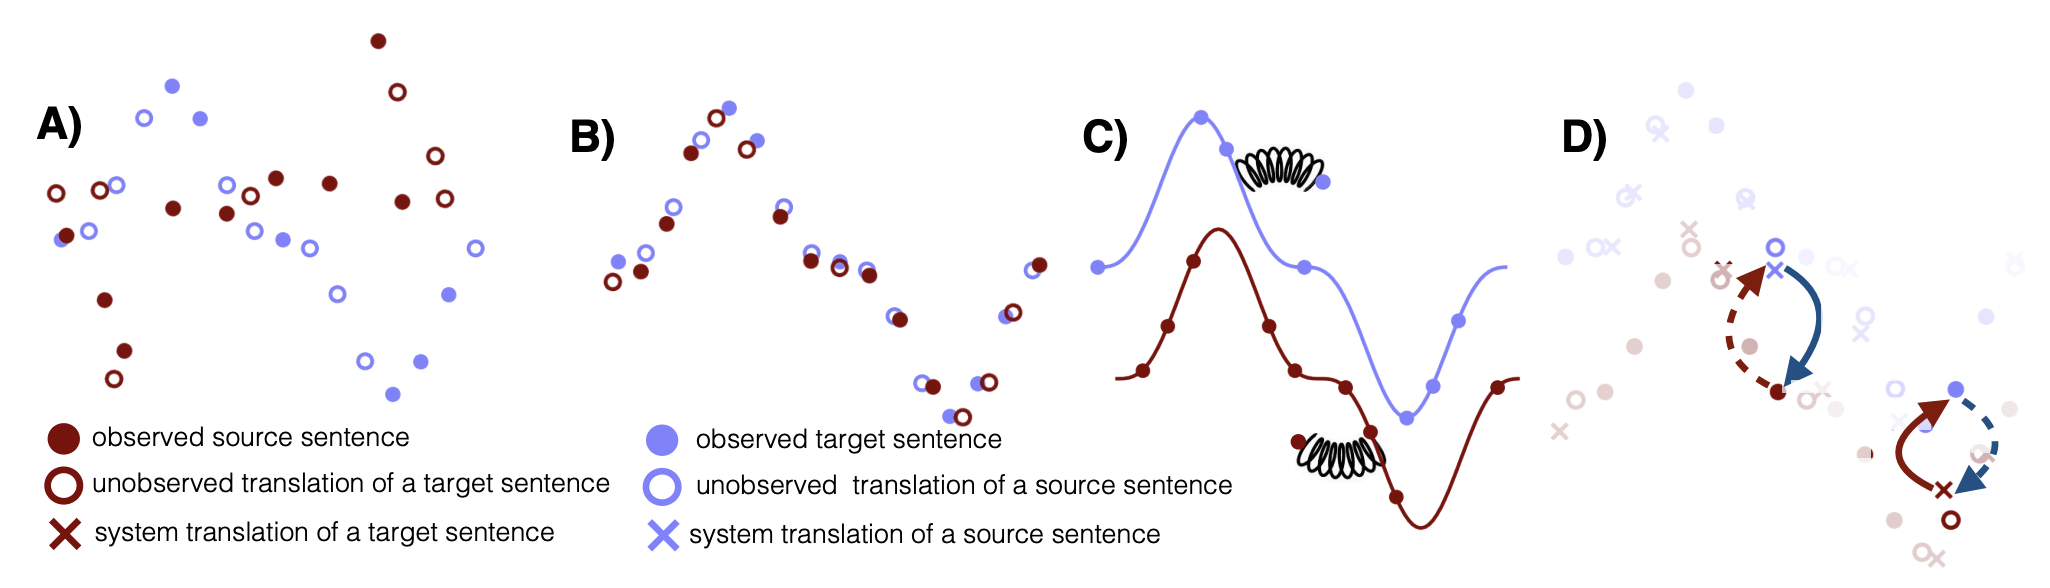
\includegraphics[width=14cm]{Images/unsupervisedNMT.png}
    \caption{Toy illustration of the three principles of unsupervised MT. Source: \cite{lample2018phrase}}
    \label{fig:unsupervisedNMT}
\end{figure}

Fig. \ref{fig:unsupervisedNMT} demonstrates the usage of the above-mentioned principals. A) There are two monolingual corpora. B) \textbf{Initialization}. The two distributions are aligned by performing word-by-word translation. C) \textbf{Language modeling}. A language model is learned independently in each domain to infer the structure in the data. D) \textbf{Back-translation}. Starting from an observed source sentence they use the current source $\rightarrow$ target model(dashed arrow), yielding a potentially incorrect translation (blue cross near the empty circle). Starting from this (back) translation, they use the target $\rightarrow$ source model (continuous arrow) to reconstruct the sentence in the original language. The discrepancy between the reconstruction and the initial sentence provides an error signal to train the target $\rightarrow$ source model parameters. The same procedure is applied in the opposite direction to train the source $\rightarrow$ target model (\cite{lample2018phrase}).

\section{XLM}
\label{sec:xlm}

Based on the ideas of aligning the distributions of sentences in different languages, \cite{lample2019cross} reduced the need for parallel data. They introduced supervised and unsupervised approaches for cross-lingual language models (XLMs\footnote{\href{https://github.com/facebookresearch/XLM}{https://github.com/facebookresearch/XLM}}) training based on Transformers' architecture~\cite{NIPS2017_7181}. The unsupervised method relies on monolingual corpora only, whereas the supervised one leverages parallel data. The XLM model achieves a better performance than the original BERT\footnote{\href{https://github.com/google-research/bert}{https://github.com/google-research/bert}} on all GLUE tasks\footnote{\href{https://github.com/facebookresearch/XLM\#i-monolingual-language-model-pretraining-bert}{https://github.com/facebookresearch/XLM\#i-monolingual-language-model-pretraining-bert}}.

\begin{figure}[h]
    \centering
    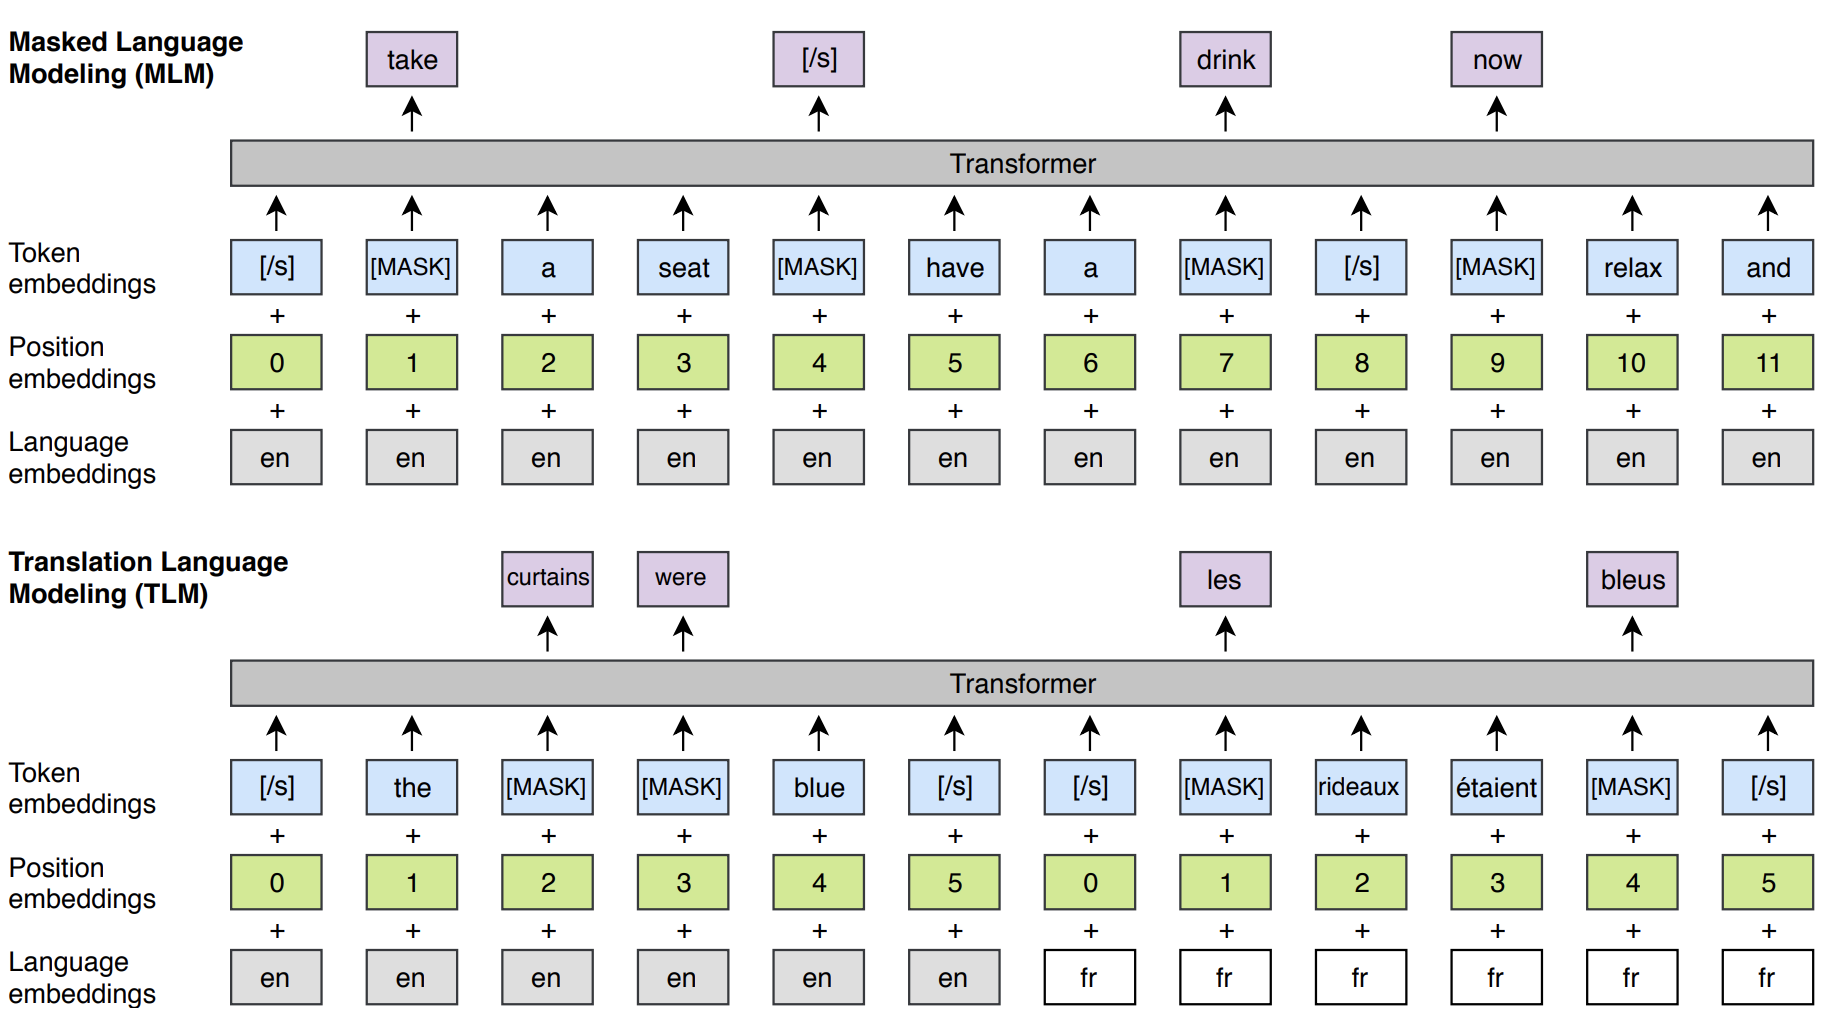
\includegraphics[width=14cm]{Images/xlm.png}
    \caption{Cross-lingual language model pretraining. Source: \cite{lample2019cross}}
    \label{fig:xlm}
\end{figure}

The unsupervised \textbf{cross-lingual text representations} are obtained with the help of \emph{Causal Language Modeling} (CLM) and \emph{Masked Language Modeling} (MLM) training objectives. During training, they process all languages with the same shared vocabulary created through Byte Pair Encoding (BPE) (\cite{Sennrich2015NeuralMT}). CLM is a Transformer language model trained to predict the probability of a word given the previous words in a sentence $P(w_{t}|w_{1}, \dots, {w_{t-1}, \Theta})$. MLM assumes random sampling of 15\% of the BPE tokens from the text streams, replacing them by a [MASK] token 80\% of the time, by a random token 10\% of the time, and keeping them unchanged 10\% of the time (fig. \ref{fig:xlm}). 

Since both the CLM and MLM only require monolingual data, they cannot be used to utilize parallel data. \emph{Translation Language Modeling} (TLM) leverages parallel corpora to improve cross-lingual pre-training. It extends the BERT MLM approach by using parallel sentences (fig. \ref{fig:xlm}). TLM randomly masks words in both the source and target sentences. To predict a word masked in a source sentence, the model can either attend to surrounding source words or to the target translation, encouraging the model to align the source and target representations. The target context can be used if the source one is not sufficient to guess the masked source words (\cite{lample2019cross}).

To the best of our knowledge, cross-lingual language modeling has not been applied before for the task of text simplification. Following this approach, we used the XLM model for our experiments.

We included the following 6 steps into the model training: CLM, TLM, \emph{Parallel Classification} (PC), \emph{Denoising Auto-Encoder} (AE), \emph{Machine Translation} (MT) and \emph{Back-translation} (BT). During the PC step, the model predicts if pairs of sentences are mutual translations of each other. AE and MT steps are similar with the only difference that for AE step the model uses mono language sentences and add noise before masking and encoding. The BT step, described in the previous section, is similar to \cite{lample2018phrase}. MT is a supervised machine translation step. In our experiments, we first consider the settings with no supervision (i.e., by excluding MT and TLM steps) and later added an MT step trained on a small parallel corpus to attest the extent to which a little supervision can help with the simplification problem. It is worth noting that the addition of TLM step, which also relies on parallel corpora, had marginal impact on the performance of the models.   

The importance of each step can be weighted by a coefficient but we did not see any improvement when changing the values of the coefficients and used the default lambdas of 1 for every step.

\section{Beam Search Generation}

Beam Search is a common technique to improve decoding performance. Instead of decoding the most probable words in a greedy fashion, it generates an output sentence by keeping a fixed number (specified by beam size parameter) of hypotheses with the highest log-probability at each step. The approach explores a set of candidate hypotheses until the sentence is fully decoded and selects the one with the highest log-probability at the end (Fig. \ref{fig:beam-search}).

\begin{figure}
    \centering
    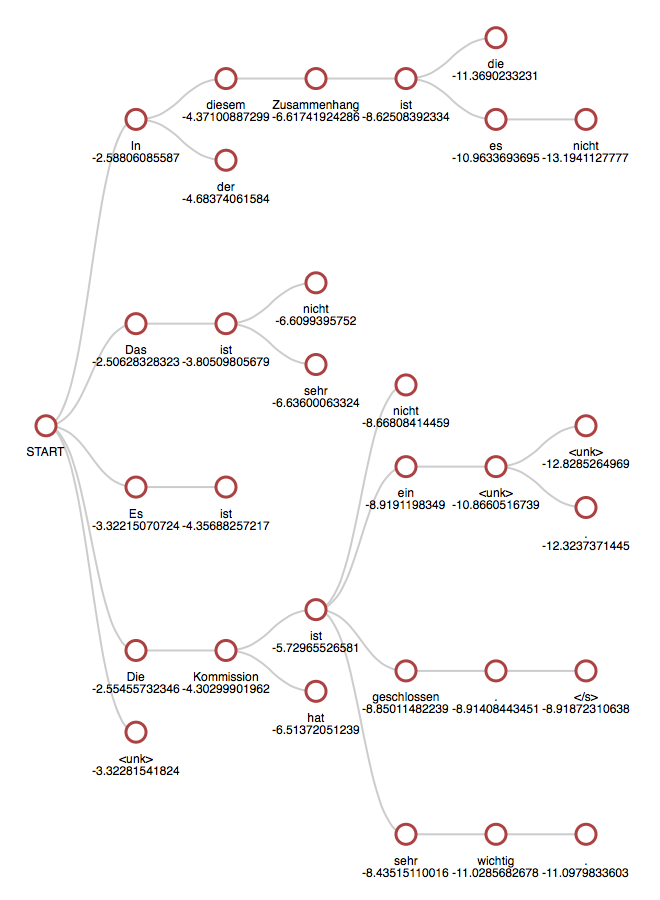
\includegraphics[width=14cm]{Images/beam_search.png}
    \caption{Visualisation of beam search of width 5. Source: OpenNMT.}
    \label{fig:beam-search}
\end{figure}

Such a decoding strategy based on scoring provides us with additional control over sentence generation. To manage the exact matches ratio, length and simplicity (FKGL-based) of a hypothesis we added three types of score penalties. 

\textbf{Length penalty} (LP) favors shorter or longer hypothesis depending on $\lambda_{length}$ parameter:
\medskip
\[LP = \lambda_{length} \times \exp(length(hypothesis))\]
\medskip

\textbf{Exact matches penalty} (EMP) uses cosine similarity between input and hypothesis to restrict copying of input:
\medskip
\[EMP = \lambda_{exact\_matches} \times \exp(cosine\_similarity(input, hypothesis))\]
\medskip

\textbf{FKGL penalty} (FKGLP) encourages hypothesis with lower FKGL score:
\medskip
\[FKGLP = \lambda_{FKGL} \times \exp(FKGL(hypothesis))\]
\medskip

We demonstrate that together these beam search penalties make it possible to improve the decoding results of a model after training.

\section{Random Subsampling Validation}

We choose random sub-sampling validation (\cite{Dubitzky}) for assessing how our models will generalize to an independent data set and for eliminating statistical errors due to dataset split. This approach belongs to \emph{non-exhaustive cross validation} methods. It does not compute all possible splits of the dataset but creates multiple random splits into training and test data (Fig. \ref{fig:subsampling}). For each such split, we train a model on training data and evaluate using test data. The final results are then averaged over the splits. The advantage of this method is that the proportion of the train/test split is not dependent on the number of partitions. The disadvantage is that test sets may overlap and some examples may never be selected. To overcome this possible problem we repeat this procedure 10 times.

\begin{figure}
    \centering
    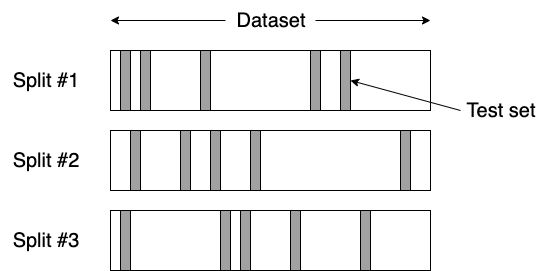
\includegraphics[width=12cm]{Images/subsampling.png}
    \caption{Repeated random subsampling. Grey areas are test data and white ares are train data.}
    \label{fig:subsampling}
\end{figure}


\section{Training Details}
\label{sec:training-details}

We trained our models on the Nvidia Tesla V100 GPU card and used the same hyper-parameters across datasets except for beam search penalty coefficients. 

Both encoder and decoder have \textbf{embedding layer of size 1024}, \textbf{6 attention layers} with \textbf{8 heads} and \textit{GELU} activation function, and regularized with an \textbf{attention dropout rate of 0.1}. 

We used \textit{Adam} optimizer with learning rate decay based on the inverse square root of the update number. \textbf{Learning rate} was set to \textbf{0.0001}, the first momentum coefficient was set to 0.9 and the second momentum coefficient to 0.98.

We examined our XLM models performance based on a range of simplification metrics discussed in Chapter \ref{chap:evaluation}. To determine which set of scores is better we introduced a new \emph{Compound Simplification Score} (CSS). Since BLEU and SARI take values from 0 to 100 (the higher the better) and FKGL takes values from 0 to 10 on our datasets (the lower the better) we defined it as follows:
\[CSS=\frac{BLEU}{100} + \frac{SARI}{100} + \frac{100 - FKGL \times 10}{100}\]

We used CSS as our stopping criteria, i.e., 5 epochs of non-increasing number. We used different epoch sizes for different datasets based on their sizes: 80,000 sentences for Newsela, 150,000 for Wikilarge and 200,000 for News/SW-CBT datasets. On average a single epoch took 15 minutes on Newsela, 35 minutes on Wikilarge and 40 minutes on News/SW-CBT datasets. All our models on all the datasets converged within 10-15 epochs.

\endinput